%%%%%%%%%%%%%%%%%%%%%%%%%%%%%%%%%%%%%%%%%%%%%%%%%%%%%%%%%%%%%%%%%%%%%%%%%%%%%%%
\subsection{Introduction}
%%%%%%%%%%%%%%%%%%%%%%%%%%%%%%%%%%%%%%%%%%%%%%%%%%%%%%%%%%%%%%%%%%%%%%%%%%%%%%%
\begin{frame}
 \begin{colorblock}{blue}{lightblue}{ }
    \Large \textbf{Introduction}
  \end{colorblock}
\end{frame}

\begin{frame}
\frametitle{Introduction and Objectives}
\begin{itemize}
	\item {\bf Hide the details of resource management}
	\begin{itemize}
		\item Let users instead focus on application developlemt
	\end{itemize}
	\item {\bf Operate applications with high reliability and availability}
	\begin{itemize}
		\item Tolerate failures within a datacenter and across datacenters
	\end{itemize}
	\item {\bf Run heterogeneous workloads and scale across thousands of machines}
\end{itemize}
\end{frame}

%%%%%%%%%%%%%%%%%%%%%%%%%%%%%%%%%%%%%%%%%%%%%%%%%%%%%%%%%%%%%%%%%%%%%%%%%%%%%%%
\subsection{User perspective}
%%%%%%%%%%%%%%%%%%%%%%%%%%%%%%%%%%%%%%%%%%%%%%%%%%%%%%%%%%%%%%%%%%%%%%%%%%%%%%%
\begin{frame}
 \begin{colorblock}{blue}{lightblue}{ }
    \Large \textbf{The User Perspective}
  \end{colorblock}
\end{frame}

\begin{frame}
\frametitle{Terminology}
\begin{itemize}
	\item Users develop applications called {\it jobs}
	\item Jobs consists in one or more {\it tasks}
	\item All tasks run the same binary
	\item Each job runs in a set of machines that are managed as a unit, called a {\it Borg Cell}
\end{itemize}
\end{frame}

\begin{frame}
\frametitle{Workloads}
\begin{itemize}
	\item {\bf Two main categories supported}
	\begin{itemize}
		\item Long-running services: jobs that should ``never'' go down, and handle short-lived, latency-sensitive requests
		\item Batch jobs: delay-tolerant jobs that can take from few seconds to few days to complete
		\item Storage services: these are long-running services like above, that are used to store data
	\end{itemize}
	\item {\bf Workload composition in a cell is dynamic}
	\begin{itemize}
		\item It varies depending on the tenants using the cell
		\item It varies with time: diurnal usage pattern for end-user-facing jobs, irregular pattern for batch jobs
	\end{itemize}
	\item {\bf Examples}
	\begin{itemize}
		\item High-priority, \texttt{production} jobs $\to$ long-running services
		\item Low-priority, \texttt{non-production} jobs $\to$ batch jobs
		\item In a typical Borg Cell
		\begin{itemize}
			\item Prod Jobs: 70\% of CPU allocation, representing 60\% of CPU usage
			\item Non-prod Jobs: 55\% of CPU allocation, representing 85\% of CPU usage
		\end{itemize}
	\end{itemize}
\end{itemize}
\end{frame}

\begin{frame}
\frametitle{Clusters and Cells}
\begin{itemize}
	\item {\bf Borg Cluster:} a set of machines connected by a high-performance datacenter-scale network fabric
	\begin{itemize}
		\item The machines in a Borg Cell all belong to a {\it single} cluster
		\item A cluster lives inside a datacenter building
		\item A collection of building makes up a {\it Site}
	\end{itemize}
	\item {\bf Borg Machines:} physical servers dedicated to execute Borg applications
	\begin{itemize}
		\item They are generally highly heterogeneous in terms of resources
		\item They may expose a public IP address
		\item They may expose advanced features, like SSD or GPGPU
	\end{itemize}
	\item {\bf Examples}
	\begin{itemize}
		\item A typical cluster usually hsts one large cell and a few small-scale test cells
		\item The {\it median cell size} is about 10 k machines
		\item Borg uses those machines to schedule application tasks, install their binaries and dependencies, monitor their health and restarting them if they fail
	\end{itemize}
\end{itemize}
\end{frame}

\begin{frame}
\frametitle{Jobs and Tasks}
\begin{itemize}
	\item {\bf Job Definition}
	\begin{itemize}
		\item Name, owner and number of tasks
		\item {\it Constraints} to force tasks run on machines with particular {\it attributes}
		\item Constraints can be {\bf hard} or {\bf soft} ({\it i.e.}, preferences)
		\item Each task maps to a set of UNIX processes running in a container on a Borg machine in a Borg Cell
	\end{itemize}
	\item {\bf Task Definition}
	\begin{itemize}
		\item Task index within their parent job
		\item Resource requirements
		\item Generally, all tasks have the {\it same} definition
		\item Tasks can run on {\bf any resource dimension}: there are no fixed-size slots or buckets
	\end{itemize}
\end{itemize}
\end{frame}

\begin{frame}
\frametitle{Jobs and Tasks}

\begin{itemize}
	\item {\bf The Borg Configuration Language}
	\begin{itemize}
		\item Declarative language to specify jobs and tasks
		\item Lambda functions to allow calculations
		\item Some application descriptions can be over 1 k lines of code
	\end{itemize}
	\item {\bf User interacting with live jobs}
	\begin{itemize}
		\item This is achieved mainly using RPC
		\item Users can update the specification of tasks, while their parent job is running
		\item Updates are non-atomic, executed in a rolling-fashion
	\end{itemize}
	\item {\bf Task updates ``side-effects''}
	\begin{itemize}
		\item Always require restarts: e.g., pushing a new binary
		\item Might require migration: e.g., change in specification
		\item Never require restarts nor migrations: e.g., change in priority
	\end{itemize}
\end{itemize}
\end{frame}

\begin{frame}
\frametitle{Jobs State Diagram}
\begin{figure}[h]
  \centering
  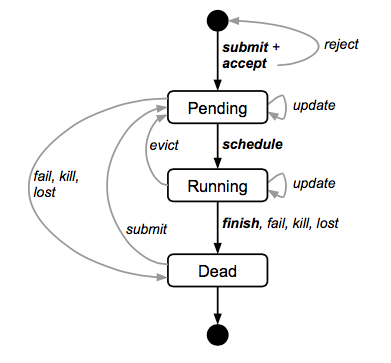
\includegraphics[scale=0.5]{./figures/borg_state_diagram}
  \label{fig:borg_state_diagram}
\end{figure}
\end{frame}

\begin{frame}
\frametitle{Resource Allocations}
\begin{itemize}
	\item {\bf The Borg ``Alloc''}
	\begin{itemize}
		\item Reserved set of resources on a machine
		\item Can be used to execute one or more tasks, that equally share resources
		\item {\bf Resources remain assigned whether or not they are used}
	\end{itemize}
	\item {\bf Typical use of Borg Allocs}
	\begin{itemize}
		\item Set resources aside for future tasks
		\item Retain resources between stopping and starting tasks
		\item Consolidate (gather) tasks from different jobs on the same machine
	\end{itemize}
	\item {\bf Alloc Sets}
	\begin{itemize}
		\item Group of allocs on different machines
		\item Once an alloc set has been created, one or more jobs can be submitted
	\end{itemize}
\end{itemize}
\end{frame}

\begin{frame}
\frametitle{Priority, Quota and Admission Control}
\begin{itemize}
	\item {\bf Mechanisms to deal with resource demand and offer}
	\begin{itemize}
		\item What to do when more work shows up than can be accommodated?
		\item Note: this is not {\it scheduling}, it is more admission control
	\end{itemize}
	\item {\bf Job priority}
	\begin{itemize}
		\item Non-overlapping {\it priority bands} for different uses
		\item This essentially means users must ``manually'' cluster their applications according to such bands
		\item[$\to$] Tasks from high-priority jobs can preempt low-priority tasks
		\item Cascade preemption is avoided by disabling it for same-band jobs
	\end{itemize}
	\item {\bf Job/User quotas}
	\begin{itemize}
		\item Used to decide which job to admit for scheduling
		\item Expressed as a vector of resource quantities
	\end{itemize}
	\item {\bf Pricing}
	\begin{itemize}
		\item Underlying mechanism to regulate user behavior
		\item Aligns user incentives to better resource utilization
		\item Discourages over-buying by over-selling quotas at lower priority
	\end{itemize}
\end{itemize}
\end{frame}

\begin{frame}
\frametitle{Naming Services}
\begin{itemize}
	\item {\bf Borg Name Service}
	\begin{itemize}
		\item A mechanism to assign a name to tasks
		\item Task name = Cell name, job name and task number
	\end{itemize}
	\item {\bf Uses the Chubby coordination service}
	\begin{itemize}
		\item Writes task names into it
		\item Writes also health information and status
		\item Used by Borg RPC mechanism to establish communication endpoints
	\end{itemize}
	\item {\bf DNS service inherits from BNS}
	\begin{itemize}
		\item Example: the 50th task in job ``jfoo'' owned by user ``ubar'' in a Borg Cell called ``cc''
		\item \texttt{50.jfoo.ubar.cc.borg.google.com}
	\end{itemize}
\end{itemize}
\end{frame}

\begin{frame}
\frametitle{Monitoring Services}
\begin{itemize}
	\item {\bf Every task in Borg has a built-in HTTP server}
	\begin{itemize}
		\item Provides health information
		\item Provides performance metrics
	\end{itemize}
	\item {\bf Borg SIGMA}
	\begin{itemize}
		\item Monitoring UI Service
		\item State of jobs, of cells
		\item Drill-down to task level
		\item {\bf Why pending?}
		\begin{itemize}
			\item ``Debugging'' service
			\item Helps users with finding job specifications that can be easily scheduled
		\end{itemize}
	\end{itemize}
	\item {\bf Billing services}
	\begin{itemize}
		\item Use monitoring information to compute usage-based charging
		\item Help users debug their jobs
		\item Used for capacity planning
	\end{itemize}
\end{itemize}
\end{frame}
